\documentclass[a4paper,14pt]{extreport}
\usepackage[utf8]{inputenc}
\usepackage[T2A]{fontenc}
\usepackage[russian]{babel}
\usepackage{eufrak}
% поля:
\usepackage[left=1cm, right=1cm, top=2cm, bottom=2cm]{geometry}
\linespread{1}
\usepackage{indentfirst} % отделять первую строку раздела абзацным отступом
\setlength\parindent{5ex}
\addto{\captionsrussian}{\renewcommand*{\contentsname}{Содержание}}
\usepackage[hidelinks]{hyperref} % гиперссылки в содержании
\usepackage{graphicx}
\usepackage{float}
\usepackage{amsmath}
\renewcommand*{\thesection}{\arabic{section}}

\usepackage{multirow}
\usepackage[normalem]{ulem}
\useunder{\uline}{\ul}{}

\usepackage{cmap}%позволяет копировать кириллицу из скомпилированного файла

% Глубина разделов, попадающих в содержание
\setcounter{tocdepth}{2}

\linespread{1.3} % настройка межстрочного интервала
\tolerance=1000 % настройка чувствительности вставки переносов
\hfuzz=0pt
\sloppy

\begin{document}
% Переменование "Список литературы" в "Литература"
\renewcommand{\refname}{Литература}
\begin{titlepage}
	\begin{center}
		\large
		МИНИСТЕРСТВО ОБРАЗОВАНИЯ И НАУКИ\\ РОССИЙСКОЙ ФЕДЕРАЦИИ
		
		\textbf{Федеральное агентство по образованию}
		\vspace{0.5cm}
		
		УНИВЕРСИТЕТ ИТМО
		\vspace{0.25cm}
		
		Факультет компьютерных технологий и управления
		
		Кафедра систем управления и информатики
		\vfill
		
		
		Студент: Артемов Кирилл\\
		группа P4135\\
		
		\textsc{\LARGE Домашнее задание № 2}\\[5mm]
		
		{\LARGE Вывод уравнений движения плоского двухзвенного маятника на основе метода Ньютона-Эйлера и численная реализация в рекуррентном виде}	\bigskip
		
	\end{center}
	\vfill
	
	\newlength{\ML}
	\settowidth{\ML}{«\underline{\hspace{0.7cm}}» \underline{\hspace{1cm}}}
	\hfill\begin{minipage}{0.4\textwidth}
		Преподаватель\\
		\underline{\hspace{\ML}} С.\,А.~Колюбин\\
		«\underline{\hspace{0.7cm}}» \underline{\hspace{2cm}} 2016 г.
	\end{minipage}%
	\bigskip
	
	\vfill
	
	\begin{center}
		Санкт-Петербург, 2016 г.
	\end{center}
\end{titlepage}

\tableofcontents
\newpage

\section{Задание}

\begin{enumerate}
	\item Вывести аналитически уравнения движения плоского двухзвенного маятника (рисунок 1) на основе метода Ньютона-Эйлера;
	\item Разработать программу, реализующую полученную динамическую
	модель робота для решения обратной задачи динамики (численная реализация уравнений Ньютона-Эйлера в рекуррентном виде).
\end{enumerate}

\begin{figure}[H]
	\center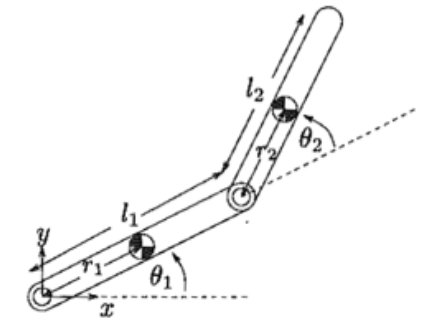
\includegraphics[width=0.5\linewidth]{images/1.png}
	\caption{Плоский двухзвенный маятник: 2 вращательных сочленения. Оба звена -- цилиндрические стержни.}
	\label{fig:scr1}
\end{figure}
На рисунке 1: $l_1, l_2$ -- длины звеньв, $r_1, r_2$ -- расстояния от начала звена до центра масс каждого из звеньев, $\theta_1, \theta_2$ -- углы поворота звеньев.

\section{Вывод уравнений движения}

\subsection{Инициализация}

Звенья вращательые, следователньо ообщенные координаты $q_i$ это $\theta_i$.

Входные данные: $q, \dot q, \dot q$ -- траектория движения, $l_1, l_2, r_1, r_2, d^{link}_1,  d^{link}_2$ -- геометричческие параметры, $m1, m2, I_i$ -- динамические параметры.

Первым делом прикрепим системы координат к маятнику в соответсвии с методом Денавита-Хартенберга как показано на рисунке 2.

\begin{figure}[H]
	\center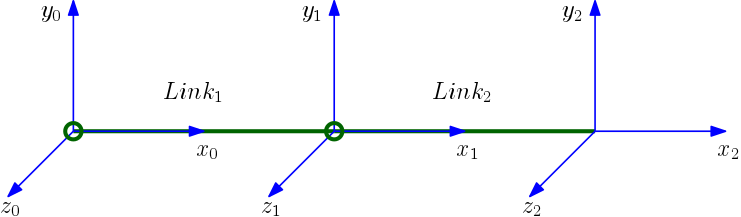
\includegraphics[width=0.8\linewidth]{images/2.png}
	\caption{Системы координат по методу ДХ}
	\label{fig:scr1}
\end{figure}

Составим таблицу 1 с параметрами ДХ.

\begin{table}[H]
	\centering
	\caption{Параметры ДХ}
	\label{my-label}
	\begin{tabular}{|c|l|l|l|l|}
		\hline
		№ & $a_i$ & $\alpha_i$ & $d_i$ & $\theta_i$ \\ \hline
		1 & $l_1$ & 0 & 0 & 0 \\ \hline
		2 & $l_2$ & 0 & 0 & 0 \\ \hline
	\end{tabular}
\end{table}

Матрицы поворота:

\begin{equation}
	^0R_1 =
	\begin{bmatrix}
		cos(q_1) & -sin(q_1) & 0\\
		sin(q_1)& cos(q_1) &0 \\
		0&0 &1
	\end{bmatrix}
\end{equation}

\begin{equation}
	^1R_2 =
	\begin{bmatrix}
	cos(q_2) & -sin(q_2) & 0\\
	sin(q_2)& cos(q_2) &0 \\
	0&0 &1
	\end{bmatrix}
\end{equation}


\subsection{Вывод уравнений}

\subsubsection{Расчет тензора инерции}

\begin{figure}[H]
	\center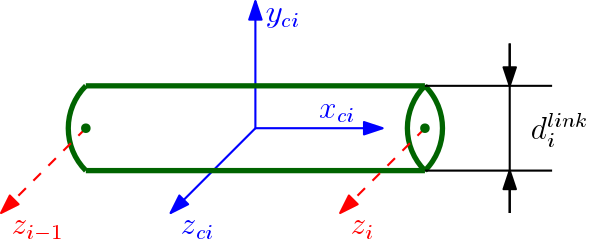
\includegraphics[width=0.8\linewidth]{images/3.png}
	\caption{Системы координат в звене}
	\label{fig:scr1}
\end{figure}
Примем за радиус $r_{link_i} = \frac{d^{link}_2}{2}$. Запишем моменты инерции для каждой из осей СК закрепленной в центре масс, как на рисунке 3. 
\begin{align}
	I_i^{xx} &= \frac{m_i r^2}{2} \\
	I_i^{yy} &= \frac{m_i (3 r_{link_i}^2 + l_i^2)}{12} \\
	I_i^{zz} &= \frac{m_i (3 r_{link_i}^2 + l_i^2)}{12}
\end{align}

Тензор инерции примет вид:
\begin{equation}
	I_i = 
	\begin{bmatrix}
	m_{i} r^{2} / 2 & 0 & 0 \\ 
	0 &    	m_i (3 r_{link_i}^2 + l_i^2) / 2 & 0\\
	0 & 0 & m_i (3 r_{link_i}^2 + l_i^2) / 2
	\end{bmatrix}
\end{equation}

Так как ось вращения проходит через начало звена, а не через центр, то воспользовавшись теоремой Гюйгенса - Штейнера, получим тензор инерции относительно оси вращения звена. Формула для пересчета:

\begin{equation}
	J_{ij} = I_{ij} + m (\textbf{d}^2 * \delta_{ij} -a_i a_j)
\end{equation}
где $J_{ij}$ -- элемент полученного тензора, $I_{ij}$ -- элемент исходного тензора, $\textbf{d} = (a_1, a_2, a_3)$ -- вектор смещения центра масс ($r_1, r_2$ по оси $X$ для каждого звена из рисунка 1), $\delta_{ij}$ -- символ Кронекера.

Получаем тензор инерции для оси вращения звена (начало звена):
\begin{equation}
	J_i = 
\begin{bmatrix}
m_{i} r^{2} / 2 & 0 & 0 \\ 
0 &    	m_i (3 r_{link_i}^2 + l_i^2) / 2 + m_i r_i^2 & 0\\
0 & 0 & m_i (3 r_{link_i}^2 + l_i^2) / 2 + m_i r_i^2
\end{bmatrix}
\end{equation}
где $r_i$ -- расстояние до центра масс звена $i$. Так как оба звена цилиндрические стержни, то полученный тензор инерции справедлив для обоих звеньев.

\subsubsection{Начальные условия}

\begin{align}
	n &= 2\\
	i &= 1..2\\
	g &= 9.81\\
	\omega_0 &= \dot \omega_0 =
	\begin{bmatrix}
		0&0&0
	\end{bmatrix}^T\\
	a_0 &=
	\begin{bmatrix}
0&0&0
\end{bmatrix}^T\\
	a_{0} &=
	\begin{bmatrix}
0&g&0
\end{bmatrix}^T\\
	f_{3} &=
\begin{bmatrix}
0&0&0
\end{bmatrix}^T\\
	\tau_{3} &=
\begin{bmatrix}
0&0&0
\end{bmatrix}^T
\end{align}


\subsubsection{Уравнения для прямой рекурсии}

\begin{itemize}
	\item Звено 1
	\begin{align*}
	\omega_1 = ^0R_1^T [\omega_0 + \dot q_1 z_0] =
	\begin{bmatrix}
	cos(q_1) & -sin(q_1) & 0\\
	sin(q_1)& cos(q_1) & 0\\
	0&0 &1
	\end{bmatrix}
	\begin{bmatrix}
	0\\
	0\\
	\dot q_1
	\end{bmatrix}
	=
	\begin{bmatrix}
	0\\
	0\\
	\dot q_1
	\end{bmatrix}\\
	\end{align*}
	\begin{align*}
	\dot \omega_1 = ^0R_1^T [\dot \omega_0 + \ddot q_1 z_0 + \dot q_1 \omega_0 \times z_0] = 
	\begin{bmatrix}
	cos(q_1) & -sin(q_1) & 0\\
	sin(q_1)& cos(q_1) &0\\
	0&0 &1
	\end{bmatrix}			
	\begin{bmatrix}
	0\\
	0\\
	\ddot q_1
	\end{bmatrix}
	=
	\begin{bmatrix}
	0\\
	0\\
	\ddot q_1
	\end{bmatrix}\\
	\end{align*}	
	
	\begin{align*}
	&a_1 = ^0R_1^T [a_0 + \dot \omega_1 \times ^1r_{01} + \omega_1 \times (\omega_1 \times ^1r_{01})]
	=\\
	&=
\begin{bmatrix}
cos(q_1) & -sin(q_1) & 0\\
sin(q_1)& cos(q_1) &0\\
0&0 &1
\end{bmatrix}			
	\begin{bmatrix}
	0\\
	g\\
	0
	\end{bmatrix}			
	+
	\begin{bmatrix}
	0\\
	l_1 \ddot q_1\\
	0
	\end{bmatrix}			
	+
	\begin{bmatrix}
	-l_1 \ddot 1_1^2\\
	0\\
	0		
	\end{bmatrix}			
	=
	\begin{bmatrix}
	-g sin(q_1) - l_1 \ddot q_1^2\\
	g cos(q_1) + l_1 \ddot q_1\\
	0
	\end{bmatrix}
	\end{align*}
	
	

\begin{align*}
	a_{c1} &= a_1 + \dot \omega_1 \times r_{1,c1} + \omega_1 \times (\omega_1 \times r_{1,c1})
	=
		\begin{bmatrix}
			-g sin(q_1) - l_1 \ddot q_1^2\\
			g cos(q_1) + l_1 \ddot q_1\\
			0
		\end{bmatrix}+\\
	&+
		\begin{bmatrix}
			0 & -\ddot q_1 & 0\\
			\ddot q_1 & 0 & 0\\
			0&0&0
		\end{bmatrix}
		\begin{bmatrix}
			-r_1\\
			0\\
			0
		\end{bmatrix}
	+
		\begin{bmatrix}
			0 & -\ddot q_1 & 0\\
			\ddot q_1 & 0 & 0\\
			0&0&0
		\end{bmatrix}
	\left(
		\begin{bmatrix}
			0 & -\dot q_1 & 0\\
			\dot q_1 & 0 & 0\\
			0&0&0
		\end{bmatrix}
		\begin{bmatrix}
		-r_1\\
		0\\
		0
		\end{bmatrix}
	\right) 
	=\\
	&=
	\begin{bmatrix}
	-g sin(q_1) - l_1 \ddot q_1^2\\
	g cos(q_1) + l_1 \ddot q_1\\
	0
	\end{bmatrix}
	+
	\begin{bmatrix}
	0\\
	-r_1 \ddot q_1\\
	0
	\end{bmatrix}
	+
	\begin{bmatrix}
	r_1 \dot q_1^2\\
	0\\
	0
	\end{bmatrix}
	=
	\begin{bmatrix}
	-g sin(q_1) -l_1 \ddot q_1^2 + r_1 \dot q_1^2\\
	g cos(q_1) + l_1 \ddot q_1 - r_1 \ddot q_1\\
	0
	\end{bmatrix}	
\end{align*}

	\item Звено 2
	
\begin{align*}
\omega_2 &= ^1R_2^T [\omega_1 + \dot q_2 z_1] = 
\begin{bmatrix}
cos(q_1) & -sin(q_1) & 0\\
sin(q_1)& cos(q_1) &0\\
0&0 &1
\end{bmatrix}
\left(
\begin{bmatrix}
0\\
0\\
\dot q_1
\end{bmatrix}
+
\begin{bmatrix}
0\\
0\\
\dot q_2
\end{bmatrix}
\right)
=
\begin{bmatrix}
0\\
0\\
\dot q_1 + \dot q_2
\end{bmatrix}
\end{align*}
	
\begin{align*}
\dot \omega_2 &= ^1R_2^T [\dot \omega_1 + \ddot q_2 z_1 + \dot q_2 \omega_1 \times z_1] = \\
&= 
\begin{bmatrix}
cos(q_1) & -sin(q_1) & 0\\
sin(q_1)& cos(q_1) &0\\
0&0 &1
\end{bmatrix}
\left(
\begin{bmatrix}
0\\
0\\
\ddot q_1
\end{bmatrix}
+
\begin{bmatrix}
0\\
0\\
\dddot q_2
\end{bmatrix}
+
\begin{bmatrix}
0 & -\dot q_2 \ddot q_1 & 0\\
\dot q_2 \ddot q_1 & 0 & 0\\
0 & 0 & 0
\end{bmatrix}
\begin{bmatrix}
0\\
0\\
1
\end{bmatrix}
\right)
=\\
&=
\begin{bmatrix}
0\\
0\\
\ddot q_1 + \ddot q_2
\end{bmatrix}
\end{align*}

\begin{align*}
a_2 &= ^1R_2^T a_1 + \dot \omega_2 \times ^2r_{12} + \omega_2 \times (\omega_2 \times ^2r_{11}) = \\
&=
\begin{bmatrix}
cos(q_1) & -sin(q_1) & 0\\
sin(q_1)& cos(q_1) &0\\
0&0 &1
\end{bmatrix}
\begin{bmatrix}
-g sin(q_1) - l_1 \ddot q_1^2\\
g cos(q_1) + l_1 \ddot q_1\\
0
\end{bmatrix}
+\\
&+
\begin{bmatrix}
0 & -(\ddot q_1 + \ddot q_2) & 0\\
\ddot q_1 + \ddot q_2 & 0 & 0\\
0 & 0 & 0
\end{bmatrix}
\begin{bmatrix}
-r_2\\
0\\
0
\end{bmatrix}
+\\
&+
\begin{bmatrix}
0 & -(\dot q_1 + \dot q_2) & 0\\
\dot q_1 + \dot q_2 & 0 & 0\\
0 & 0 & 0
\end{bmatrix}
\left(
\begin{bmatrix}
0 & -(\dot q_1 + \dot q_2) & 0\\
\dot q_1 + \dot q_2 & 0 & 0\\
0 & 0 & 0
\end{bmatrix}
\begin{bmatrix}
-r_2\\
0\\
0
\end{bmatrix}
\right)
=\\
&=
\begin{bmatrix}
cos(q_2) (-g sin(q_1) - l_1 \ddot q_1^2) - sin(q_2) (g cos(q_1) + l_1 \ddot q_1) + r_2 (\dot q_1 + \dot q_2)^2\\
sin(q_2) ) (-g sin(q_1) - l_1 \ddot q_1^2) - cos(q_2) (g cos(q_1) + l_1 \ddot q_1) - r_2 (\ddot q_1 + \ddot q_2)\\
0
\end{bmatrix}
\end{align*}


\begin{align*}
&a_{c2} = a_2 + \dot \omega_2 \times r_{2,c2} + \omega_2 \times (\omega_2 \times r_{2,c2}) =\\
&=
\begin{bmatrix}
cos(q_2) (-g sin(q_1) - l_1 \ddot q_1^2) - sin(q_2) (g cos(q_1) + l_1 \ddot q_1) + r_2 (\dot q_1 + \dot q_2)^2\\
sin(q_2) ) (-g sin(q_1) - l_1 \ddot q_1^2) - cos(q_2) (g cos(q_1) + l_1 \ddot q_1) - r_2 (\ddot q_1 + \ddot q_2)\\
0
\end{bmatrix}
+\\
&+
\begin{bmatrix}
0 & -(\ddot q_1 + \ddot q_2) & 0\\
\ddot q_1 + \ddot q_2 & 0 & 0\\
0 & 0 & 0
\end{bmatrix}
\begin{bmatrix}
-r_2\\
0\\
0
\end{bmatrix}
+\\
&+
\begin{bmatrix}
0 & -(\dot q_1 + \dot q_2) & 0\\
\dot q_1 + \dot q_2 & 0 & 0\\
0 & 0 & 0
\end{bmatrix}
\left(
\begin{bmatrix}
0 & -(\dot q_1 + \dot q_2) & 0\\
\dot q_1 + \dot q_2 & 0 & 0\\
0 & 0 & 0
\end{bmatrix}
\begin{bmatrix}
-r_2\\
0\\
0
\end{bmatrix}
\right)
=\\
&=
\begin{bmatrix}
cos(q_2) (-g sin(q_1) - l_1 \ddot q_1^2) - sin(q_2) (g cos(q_1) + l_1 \ddot q_1) + r_2 (\dot q_1 + \dot q_2)^2 + r_2(\dot q_1 + \dot q_2)^2\\
sin(q_2) ) (-g sin(q_1) - l_1 \ddot q_1^2) - cos(q_2) (g cos(q_1) + l_1 \ddot q_1) - r_2 (\ddot q_1 + \ddot q_2) - r_2(\ddot q_1 + \ddot q_2)\\
0
\end{bmatrix}
\end{align*}
\end{itemize}


\subsubsection{Уравнения для обратной рекурсии}

\begin{itemize}
	\item Звено 2
\begin{align*}
f_2 &= f_3 + m_2 a_{c2} =\\
&=
\begin{bmatrix}
m_2 cos(q_2) (-g sin(q_1) - l_1 \ddot q_1^2) - m_2 sin(q_2) (g cos(q_1) + l_1 \ddot q_1)\\
m_2 sin(q_2) ) (-g sin(q_1) - l_1 \ddot q_1^2) - m_2 cos(q_2) (g cos(q_1) + l_1 \ddot q_1)\\
0
\end{bmatrix}
+\\
&+
\begin{bmatrix}
m_2 r_2 (\dot q_1 + \dot q_2)^2 + m_2 r_2(\dot q_1 + \dot q_2)^2\\
m_2 r_2 (\ddot q_1 + \ddot q_2) - m_2 r_2(\ddot q_1 + \ddot q_2)\\
0
\end{bmatrix}
\end{align*}	
	

\begin{align*}
\tau_2 &= \tau_3 - f_2 \times (^2 r_{12} + r_{2,c2}) + f_3 \times r_{2c2} + J_2 \dot \omega_2 + \omega_2 \times (J_2 \omega_2) =\\
&=
\left(
\begin{bmatrix}
m_2 cos(q_2) (-g sin(q_1) - l_1 \ddot q_1^2) - m_2 sin(q_2) (g cos(q_1) + l_1 \ddot q_1)\\
m_2 sin(q_2) ) (-g sin(q_1) - l_1 \ddot q_1^2) - m_2 cos(q_2) (g cos(q_1) + l_1 \ddot q_1)\\
0
\end{bmatrix}
\right.
+\\
&+
\left.
\begin{bmatrix}
m_2 r_2 (\dot q_1 + \dot q_2)^2 + m_2 r_2(\dot q_1 + \dot q_2)^2\\
m_2 r_2 (\ddot q_1 + \ddot q_2) - m_2 r_2(\ddot q_1 + \ddot q_2)\\
0
\end{bmatrix}
\right) \times
\begin{bmatrix}
l_2 - r_2\\
0\\
0
\end{bmatrix}
+\\
&+
\begin{bmatrix}
\frac{m_{i} r^{2}}{2} & 0 & 0 \\ 
0 & \frac{m_i (3 r_{link_i}^2 + l_i^2)}{2} + m_i r_i^2 & 0\\
0 & 0 & \frac{m_i (3 r_{link_i}^2 + l_i^2)}{2} + m_i r_i^2
\end{bmatrix}
\begin{bmatrix}
0\\
0\\
\ddot q_1 + \ddot q_2
\end{bmatrix}
+\\
&+
\begin{bmatrix}
0 & -(\dot q_1 + \dot q_2) & 0\\
\dot q_1 + \dot q_2 & 0 & 0\\
0&0&0
\end{bmatrix}
\begin{bmatrix}
0\\
0\\
(\dot q_1 + \dot q_2)\frac{m_i (3 r_{link_i}^2 + l_i^2)}{2} + m_i r_i^2
\end{bmatrix}
=\\
&=
\left(
\begin{bmatrix}
m_2 cos(q_2) (-g sin(q_1) - l_1 \ddot q_1^2) - m_2 sin(q_2) (g cos(q_1) + l_1 \ddot q_1)\\
m_2 sin(q_2) ) (-g sin(q_1) - l_1 \ddot q_1^2) - m_2 cos(q_2) (g cos(q_1) + l_1 \ddot q_1)\\
0
\end{bmatrix}
\right.
+\\
&+
\left.
\begin{bmatrix}
m_2 r_2 (\dot q_1 + \dot q_2)^2 + m_2 r_2(\dot q_1 + \dot q_2)^2\\
m_2 r_2 (\ddot q_1 + \ddot q_2) - m_2 r_2(\ddot q_1 + \ddot q_2)\\
0
\end{bmatrix}
\right) \times
\begin{bmatrix}
l_2 - r_2\\
0\\
0
\end{bmatrix}
+\\
&+
\begin{bmatrix}
0\\
0\\
(\ddot q_1 + \ddot q_2)\frac{m_i (3 r_{link_i}^2 + l_i^2)}{2} + m_i r_i^2
\end{bmatrix}
\end{align*}

	\item Звено 1
	
	\begin{align*}
		f_1 &= f_2 + m_1 a_{c1}\\
		\tau_1 &= \tau_2 - f_1 \times (^1 r_{01} + r_{1,c1}) + f_2 \times r_{1c1} + J_1 \dot \omega_1 + \omega_1 \times (J_1 \omega_1)
	\end{align*}


\end{itemize}



\subsection{}


\end{document}


